% !TeX spellcheck = en_US
\PassOptionsToPackage{colorlinks=true}{hyperref}
\PassOptionsToPackage{table}{xcolor}
\documentclass[handout]{beamer}
%\usetheme{Copenhagen}
\usepackage{dsfont}
\usepackage{upgreek}
\usepackage{mathtools}
\usepackage{algorithm2e}



\title{Introduction to Boosting}
\author{Predrag Tadi\'{c}}
\institute{
	School of Electrical Engineering\\
	University of Belgrade
}
\date{PSI:ML, August 2019}

% OPERATORI
\DeclareMathOperator{\E}{E}
\DeclareMathOperator{\var}{var}
\DeclareMathOperator{\std}{std}
\DeclareMathOperator{\cov}{cov}
\DeclareMathOperator{\prob}{Pr}
\DeclareMathOperator{\med}{med}
\DeclareMathOperator{\erfc}{erfc}
\DeclareMathOperator{\erf}{erf}
\newcommand{\FT}{\ensuremath{\operatorname{\mathcal{F}}}}
\newcommand{\LT}{\ensuremath{\operatorname{\mathcal{L}}}}
\newcommand{\ZT}{\ensuremath{\operatorname{\mathcal{Z}}}}
\newcommand{\ft}[1]{\ensuremath{\operatorname{\mathcal{F}} \! \left\{ #1 \right\}}}
\newcommand{\ift}[1]{\ensuremath{\operatorname{\mathcal{F}}^{-1} \! \left\{ #1 \right\}}}
\newcommand{\lt}[1]{\ensuremath{\operatorname{\mathcal{L}} \! \left\{ #1 \right\}}}
\newcommand{\ilt}[1]{\ensuremath{\operatorname{\mathcal{L}}^{-1} \! \left\{ #1 \right\}}}
\newcommand{\zt}[1]{\ensuremath{\operatorname{\mathcal{Z}} \! \left\{ #1 \right\}}}
\newcommand{\izt}[1]{\ensuremath{\operatorname{\mathcal{Z}}^{-1} \! \left\{ #1 \right\}}}
\newcommand{\re}[1]{\ensuremath{\operatorname{Re} \! \left\{ #1 \right\}}}
\newcommand{\im}[1]{\ensuremath{\operatorname{Im} \! \left\{ #1 \right\}}}
\DeclareMathOperator{\diag}{diag}
\DeclareMathOperator{\vspan}{span}
\DeclareMathOperator{\range}{\mathcal{R}}
\DeclareMathOperator{\nullSpace}{\mathcal{N}}
\DeclareMathOperator{\adj}{adj}
\DeclareMathOperator{\tr}{tr}
\DeclareMathOperator{\rang}{rang}
\DeclareMathOperator{\rank}{rank}
\DeclareMathOperator{\card}{card}
\newcommand{\nzd}[1]{\ensuremath{\operatorname{\textsc{nzd}} \! \left\{ #1 \right\}}}
\newcommand{\nzs}[1]{\ensuremath{\operatorname{\textsc{nzs}} \! \left\{ #1 \right\}}}
\newcommand{\Ev}[1]{\ensuremath{\operatorname{Ev} \! \left\{ #1 \right\}}}
\newcommand{\Od}[1]{\ensuremath{\operatorname{Od} \! \left\{ #1 \right\}}}
\newcommand{\mv}[1]{\ensuremath{\mathrm{\mathbf{#1}}}}   % matrice i vektori
\newcommand{\mvt}[1]{\ensuremath{\mathrm{\mathbf{#1}}(t)}}   % vektorske f-je vremena
\newcommand{\mvh}[1]{\ensuremath{\hat{\mathrm{\mathbf{#1}}}}}   % matrice i vektori sa kapicom (estimacije)
\newcommand{\mvht}[1]{\ensuremath{\hat{\mathrm{\mathbf{#1}}}(t)}}   % matrice i vektori sa kapicom (estimacije) i argumentom (t)
\newcommand{\mvs}[1]{\ensuremath{\boldsymbol{#1}}}       % grcke matrice i vektori (symbol)
\newcommand{\mvst}[1]{\ensuremath{\boldsymbol{#1}(t)}}       % grcke matrice i vektori (symbol) sa argumentom (t)
\newcommand{\mvsh}[1]{\ensuremath{\hat{\boldsymbol{#1}}}}       % grcke matrice i vektori (symbol) sa kapicom
\newcommand{\mvsht}[1]{\ensuremath{\hat{\boldsymbol{#1}}(t)}}       % grcke matrice i vektori (symbol) sa kapicom i argumentom (t)


\newcommand{\jdn}[1]{\ensuremath{\,\mathrm{#1}}}         % jedinice
\newcommand{\unt}[1]{\ensuremath{\,\mathrm{#1}}}         % units
%\newcommand{\dd}{\ensuremath{\, d}}                      % d u integralu
\newcommand{\dd}{\ensuremath{\, \mathrm{d}}}                      % d u integralu
\newcommand{\od}{\ensuremath{\mathrm{d}}}                 % operator diferenciranja
\DeclareMathOperator{\sinc}{sinc}
\DeclareMathOperator{\sgn}{sgn}
\DeclareMathOperator{\sign}{sign}
\DeclareMathOperator{\kullInf}{K}                        % Kullback-Leibler information
\DeclareMathOperator{\kullDiv}{J}                        % Kullback-Leibler divergence
\DeclareMathOperator{\fishInf}{I}                        % Fisher information
\DeclareMathOperator{\FishInf}{\mathcal I}               % Fisher information
\DeclareMathOperator{\fishInfM}{\mv{I}}                  % Fisher information matrix
\DeclareMathOperator{\FishInfM}{\mv{I}}                  % Fisher information matrix
\DeclareMathOperator{\dist}{P}                           % distribution
\DeclareMathOperator{\distOf}{\mathcal{L}}               % distribution
\DeclareMathOperator{\shanEnt}{N}                        % Shannon entropy
\DeclareMathOperator{\mse}{mse}                          % mean-squared error
\DeclareMathOperator{\bmse}{Bmse}
\DeclareMathOperator{\Bmse}{Bmse}
\DeclareMathOperator{\crlb}{crlb}                        % Cramer-Rao lower bound
\DeclareMathOperator{\normDist}{\mathcal{N}}             % normal distribution
\DeclareMathOperator{\unifDist}{\mathcal{U}}             % uniform distribution
\DeclareMathOperator{\PoisDist}{Poisson}             	% Poisson distribution
\DeclareMathOperator{\BernDist}{Bernoulli}             	
\DeclareMathOperator{\expFam}{ExpFam}           		 % eksponencijalna familija
\DeclareMathOperator{\bernDist}{Bernoulli}        		 % Bernulijeva raspodela
\DeclareMathOperator{\VC}{VC}							% VC dimenzija
\newcommand{\cba}[3]{\ensuremath{\overset{#3}{\underset{#2}{#1}}}}   % center_bellow^above
%\DeclareMathOperator*{\Res}{Res}                   % residue
\DeclareMathOperator{\ent}{\mathcal{E}}            % entropy
\newcommand{\tp}{\mathsf{T}}                       % transposed
%\newcommand{\tp}{\mathrm{T}}                       % transposed
\newcommand{\herm}{\mathsf{H}}                     % Hermitian (transposed and conjugated)
\DeclareMathOperator{\cost}{\mathcal{C}}
\DeclareMathOperator{\risk}{\mathcal{R}}
\DeclareMathOperator{\loss}{\mathcal{L}}
\DeclareMathOperator*{\argmax}{arg\,max}
\DeclareMathOperator*{\argmin}{arg\,min}
\newcommand{\snr}{\mathrm{SNR}}
\newcommand{\hypo}{\ensuremath{\mathcal{H}}}       % hypothesis
\DeclareMathOperator*{\esssup}{esssup}		   % essential supremum (almost everywhere)
\newcommand{\asymDist}{\ensuremath{\stackrel{a}{\sim}}} % asymptotic distribution
\newcommand{\Sgm}[2]{\ensuremath{\mvs\Sigma_{\mv{#1#2}}}}    % kovarijaciona matrica
\newcommand{\Sgmh}[2]{\ensuremath{\hat{\mvs\Sigma}_{\mv{#1#2}}}}    % procenjena kovarijaciona matrica
\newcommand{\niz}[2]{\ensuremath{#1\colon\!#2}}    % низ одбирака са индексима од #1 до #2
\newcommand{\cond}{\ensuremath{\,|\,}}
\newcommand{\indFun}[1]{\ensuremath{\mathds{1}_{#1}}}         % indicator fun.
\DeclareMathOperator{\bigO}{\mathcal O}
\DeclareMathOperator{\proj}{proj}


% Za manji tekst u hiperlinkovima
\newcommand{\hreftextsize}{\footnotesize}
\newcommand{\myhref}[2]{\href{#1}{\hreftextsize #2}}

\renewcommand{\indFun}{\ensuremath{\mathds{1}}}

\setbeamertemplate{navigation symbols}{}	%remove navigation symbols

% za broj slajda u donjem desnom uglu:
\setbeamertemplate{sidebar right}{}
\setbeamertemplate{footline}{%
	\hfill
	%\usebeamertemplate***{navigation symbols}\hspace{1cm}
	\insertframenumber%{}\hspace{2mm}\vspace{2mm}
	/\inserttotalframenumber{}\hspace{2mm}\vspace{2mm}
}

%% za više slajdova po stranici
%\usepackage{pgfpages}
%\pgfpagesuselayout{4 on 1}[a4paper, border shrink = 5mm, landscape] %[letterpaper, border shrink = 5mm, landscape]

% Za otkrivanje stavki jedna-po-jedna
\setbeamercovered{transparent=50}	% delimično sakrivanje neaktivnih delova
\setbeamercovered{still covered={\opaqueness<1->{0}}, 
	again covered={\opaqueness<1->{30}}}


%======================================================================

\begin{document}

\begin{frame}
	\titlepage
\end{frame}

\begin{frame}{Outline}
	\tableofcontents
\end{frame}

\section{Terminology}

\begin{frame}{Ensemble (committee)}
	\centering
	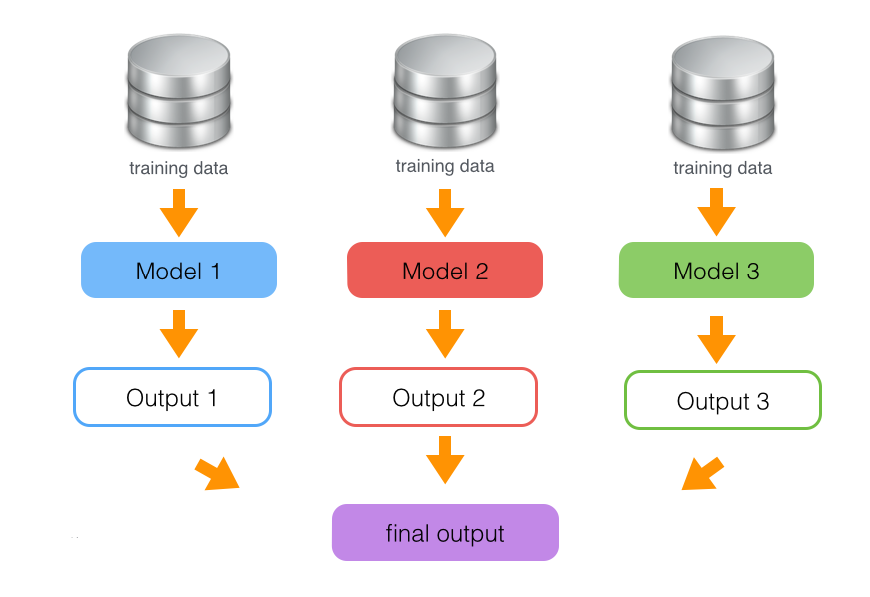
\includegraphics[width=\textwidth]{figs/ensemble}
	\\
	\myhref{https://blog.dataversioncontrol.com/ml-model-ensembling-with-fast-iterations-91e8cad6a9b5}{[dataversioncontrol.com]}
\end{frame}

\begin{frame}{Bootstraping}
\begin{itemize}
	\item Sampling $ N $ out of $ N $ with replacement, $ M $ times.
	\item $ 30\% $ of examples are not chosen in each sample.
\end{itemize}
	\centering
	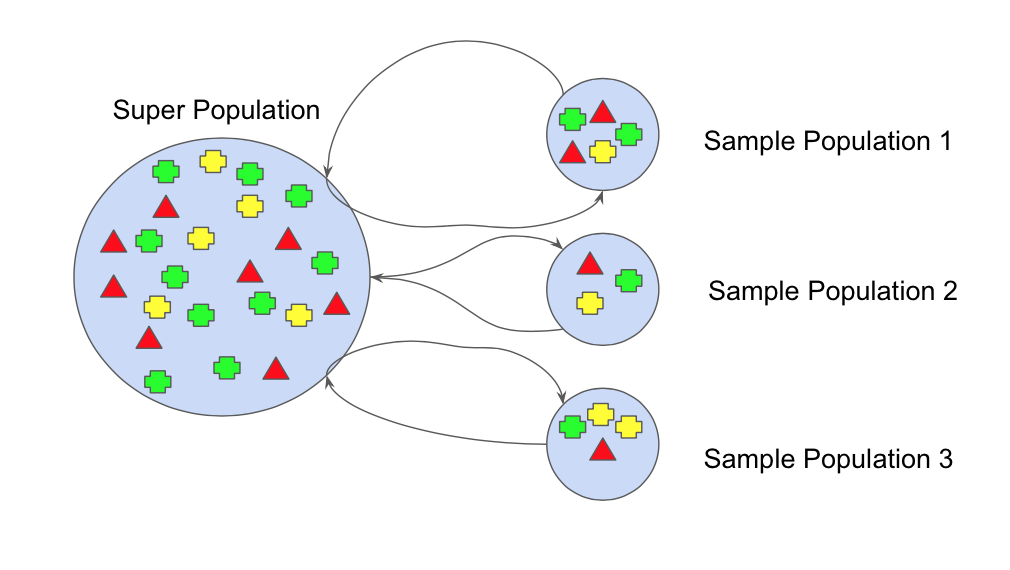
\includegraphics[width=\textwidth]{figs/bootstraping}
	\\
	\myhref{https://hackernoon.com/how-to-develop-a-robust-algorithm-c38e08f32201}{[hackernoon.com]}
\end{frame}

\begin{frame}{Weak learner, strong learner}
\begin{description}
	\item[Weak learner] simple classifier, slightly better than guessing
	\item[Strong learner] can achieve arbitrary accuracy with enough data
\end{description}
\begin{center}
	
\includegraphics[width=0.8\textwidth]{figs/good_bad_student}
	\\
	{\hreftextsize[Kidsday staff artist / Maggie Flaherty, Merrick]}
\end{center}
\end{frame}

\begin{frame}{Weak learner, strong learner}{In the PAC framework}
\begin{itemize}[<+>]
\item Notation\\
\begin{tabular}{cl}
	$ \{\mv x_i, y_i\}_{i=1}^N $ & training set \\
	$ P $ & distribution of training set \\
	$ f(\mv x) = y $ & true hypothesis \\
	$ h(\mv x) = \hat y $ & learned hypothesis \\
	$ \Pr_P\left[h(\mv x)\ne f(\mv x)\right] $ & generalization error
\end{tabular}

\item Strong learner (SL)
\begin{itemize}[<.->]
	\item for any $ P, f, \delta, \epsilon\ge 0$
	\item for large enough $ N $
	\item outputs a classifier with $ \Pr_{P}\left[h(\mv x) \ne f(\mv x)\right] \le \epsilon $
	\item with probability at least $ 1-\delta $
\end{itemize}

\item Weak learner (WL)
\begin{itemize}[<.->]
	\item for any $ P, f, \delta $ and \alert{some} $ 0\le \epsilon < 1/2 $
	\item for large enough $ N $
	\item outputs a classifier with $ \Pr_{P}\left[h(\mv x) \ne f(\mv x)\right] \le \epsilon $
	\item with probability at least $ 1-\delta $
\end{itemize}
\end{itemize}
\end{frame}

\begin{frame}{Bagging \& Boosting: training}
%\begin{itemize}
%	\item Bagging (bootstrap aggregation)
%	\begin{itemize}
%		\item \alert{parallel training} of WLs on bootstraped datasets
%		\item \alert{democratic voting}: all WLs have \alert{equal weight}
%		\item famous example: \alert{Random Forest}
%	\end{itemize}
%
%	\item Boosting
%	\begin{itemize}
%		\item \alert{sequential training} of WLs
%		\item each WL focuses on examples that previous WLs got wrong
%		\item \alert{weighted voting}: WLs can have different weights
%		\item famous examples: \alert{AdaBoost}, XGBoost
%	\end{itemize}
%\end{itemize}

%\begin{table}
%\rowcolors{1}{white}{blue!10}
%\begin{tabular}{l|lp{5cm}}
%	\rowcolor{blue!40} & Bagging & Boosting \\\hline\hline
%	Datasets & bootstraped & focus on misclassified examples \\
%	Training & parallel & sequential \\
%	Voting & democratic & weighted \\
%	Methods & Random Forest & AdaBoost
%\end{tabular}
%\end{table}
%\vfill
\begin{center}
	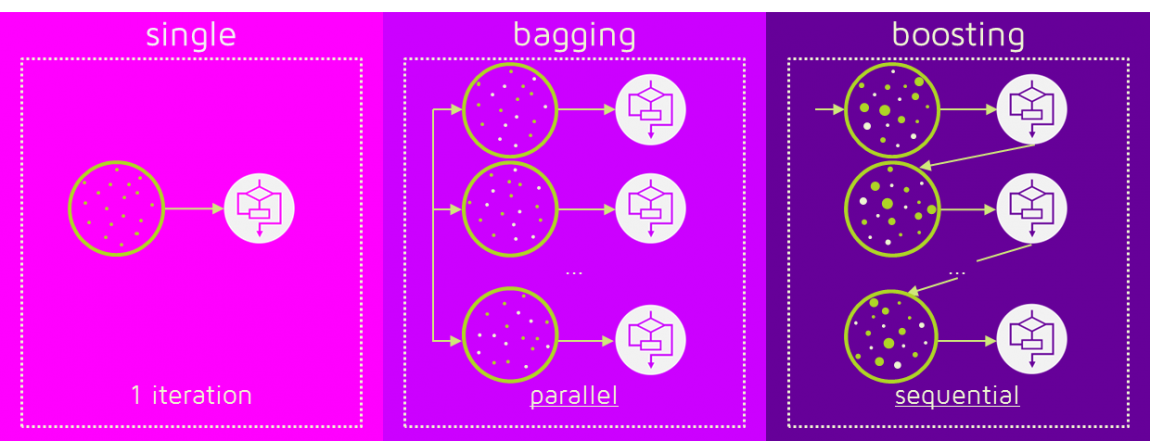
\includegraphics[width=\textwidth]{figs/bagg_boost_train}
	
	\myhref{https://quantdare.com/what-is-the-difference-between-bagging-and-boosting/}{[quantdare.com]}
\end{center}
\end{frame}

\begin{frame}{Bagging \& Boosting: decision}
\begin{center}
	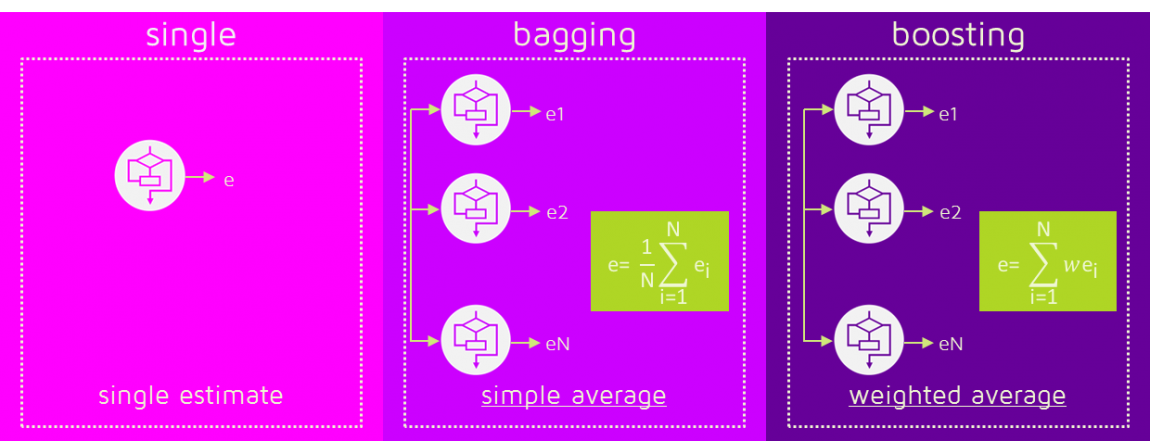
\includegraphics[width=\textwidth]{figs/bagg_boost_decide}
	
	\myhref{https://quantdare.com/what-is-the-difference-between-bagging-and-boosting/}{[quantdare.com]}
\end{center}
\end{frame}



\section{History}

\begin{frame}{History}
\begin{itemize}
	\item[1989] Does weak learnability imply strong learnability \cite{KearnsValiant1994}?
	
	\item[1990] 3 weak learners on 3 modified distributions \cite{Schapire1990}
	
	\item[1995] Boosting by majority \cite{Freund1995}
	
	\item[1996] AdaBoost \cite{FreundSchapire1996}
	
	\item[2001] Gradient Boosting \cite{Friedman2001}
	
	\item[2016] XGBoost \cite{ChenGuestrin2016}
\end{itemize}
\end{frame}

\begin{frame}{First boosting algorithm \cite{Schapire1990}}
\begin{itemize}
	\item Requires a continuous stream of labeled data.
	\item Learns 3 hypothesis on 3 modified distributions.
	\item Outputs their majority vote.
	\item Algorithm:
	\begin{enumerate}[<+>]
		\item Randomly choose first first $ N $ samples. \\
		Use them to learn $ h_1 $.
		\item Choose next batch so that $ N/2 $ samples are misclassified by $ h_1 $. \\ Use it to learn $ h_2 $.
		\item Choose next batch of $ N $ samples so that $ h_1 $ and $ h_2 $ disagree.\\
		Use it to learn $ h_3 $.
		\item Apply recursively.
	\end{enumerate}
\end{itemize}
\end{frame}



\section{AdaBoost}
\begin{frame}{AdaBoost}
\begin{center}
	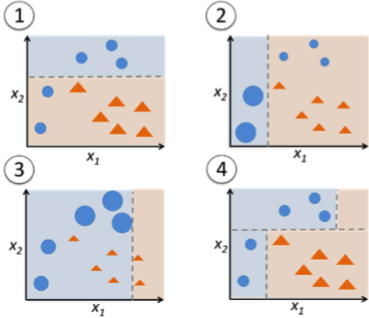
\includegraphics[width=0.7\textwidth]{figs/boosting_cr}

	\myhref{https://sebastianraschka.com/faq/docs/bagging-boosting-rf.html}{[sebastianraschka.com]}
\end{center}
\end{frame}

\begin{frame}{AdaBoost}{Preliminaries}
\begin{center}
\begin{tabular}{cl}
	%$ \{ \mv x_i, y_i \}_{i=1}^m $ & training set \\
	$ h_l(\mv x) $ & $ l $-th WL, $ h_l(\mv x) = \pm 1 $ (e.g.\ stump or perceptron) \\
	$ \alpha_l $ & voting weight of $ l $-th WL \\
	$ \omega_{l, i} $ & weight of $ i $-th example in $ l $-th iteration, $ \sum_{i=1}^N \omega_{l, i} = 1 $
\end{tabular}
\end{center}
\begin{itemize}[<+(1)->]
%	\item Sample weights are normalized: $ \sum_{i=1}^m \omega_l^{(i)} = 1 $
	
	\item Hypothesis (strong learner) after $ k $ iterations
	\begin{gather*}
		H_k(\mv x) = \frac{1}{2} \sum\nolimits_{l=1}^k \alpha_l h_l(\mv x)
	\end{gather*}
	
	\item In iteration $ k $, min exponential loss \alert{w.r.t. $ \alpha_k $ and $ h_k(\mv x) $ only}
	\begin{align*}
		E_k &= \sum\nolimits_{i=1}^N \exp\left[
			-y_i H_k(\mv x_i)
		\right]
		\\
		&= \sum\nolimits_{i=1}^N
			\underbrace{\exp\left[-y_i H_{k-1}(\mv x_i)\right]}_{\omega_{k, i}}
			\exp\left[-\frac{1}{2}y_i\alpha_k h_k(\mv x_i)\right]
	\end{align*}
\end{itemize}
\end{frame}

\begin{frame}{AdaBoost}{Training}
\begin{itemize}
	\item<1> Initialization: $ \omega_{1, 1} = \cdots = \omega_{1, N} = 1/N $
	\item<2-> For $ k = 1, \ldots, K $ (until convergence)
	\begin{enumerate}
		\item<2-3> Train weak learner
		\onslide<3->{\begin{gather*}
		\text{choose $ h_k $ to minimize }
		J_k = \sum\nolimits_{i=1}^N \omega_{k, i} \indFun\{h_k(\mv x_i) \ne y_i\}
		\end{gather*}}
		
		\item<2,4> Compute its voting weight
		\onslide<4->{\begin{align*}
		\epsilon_k &= \sum\nolimits_{i=1}^N \omega_{k, i}
			\indFun\left\{ h_k(\mv x_i) \ne y_i \right\}
		\tag{\text{weighted error}}
		\\
		\alpha_k &= \ln\frac{1-\epsilon_k}{\epsilon_k}
		\tag{\text{voting weight}}
		\end{align*}}
		
		\item<2,5> Update sample weights for next iteration
		\onslide<5->{\begin{gather*}
		\omega_{k+1, i} \propto \omega_{k, i}
		e^{\alpha_k \indFun\left\{ h_k(\mv x_i) \ne y_i \right\}},
		\qquad
		\sum\nolimits_{i=1}^N \omega_{k+1, i} = 1
		\end{gather*}}
	\end{enumerate}
\end{itemize}
\end{frame}

\begin{frame}{AdaBoost}{Convergence}
\begin{itemize}[<+>]
	\item Loss is an upper limit on training error
	\begin{gather*}
		\hat\epsilon_k \triangleq
		\frac{1}{N} \sum_{i=1}^N \indFun\left\{ 
			H_k\left(\mv x_i\right) y_i < 0
		\right\}
		\le \frac{E_k}{N}
	\end{gather*}
	
	\item If weighted error is $ \le \frac{1}{2}-\delta $ for each WL
	\begin{gather*}
		E_k \le \sqrt{1-4\delta^2} E_{k-1} \le \left(
			1-4\delta^2
		\right)^{k/2} N
		\qquad
		(E_0 \le N)
	\end{gather*}
	
	\item Both the loss and the training error are always decreasing!
	
	\item Zero training error after finite number of iterations
	\begin{gather*}
		\hat\epsilon_k = 0 \quad \text{for} \quad
		k \ge -2\frac{\ln N}{\ln (1-4\delta^2)}
	\end{gather*}
\end{itemize}
\end{frame}

\begin{frame}{AdaBoost}{Convergence}
\begin{center}
	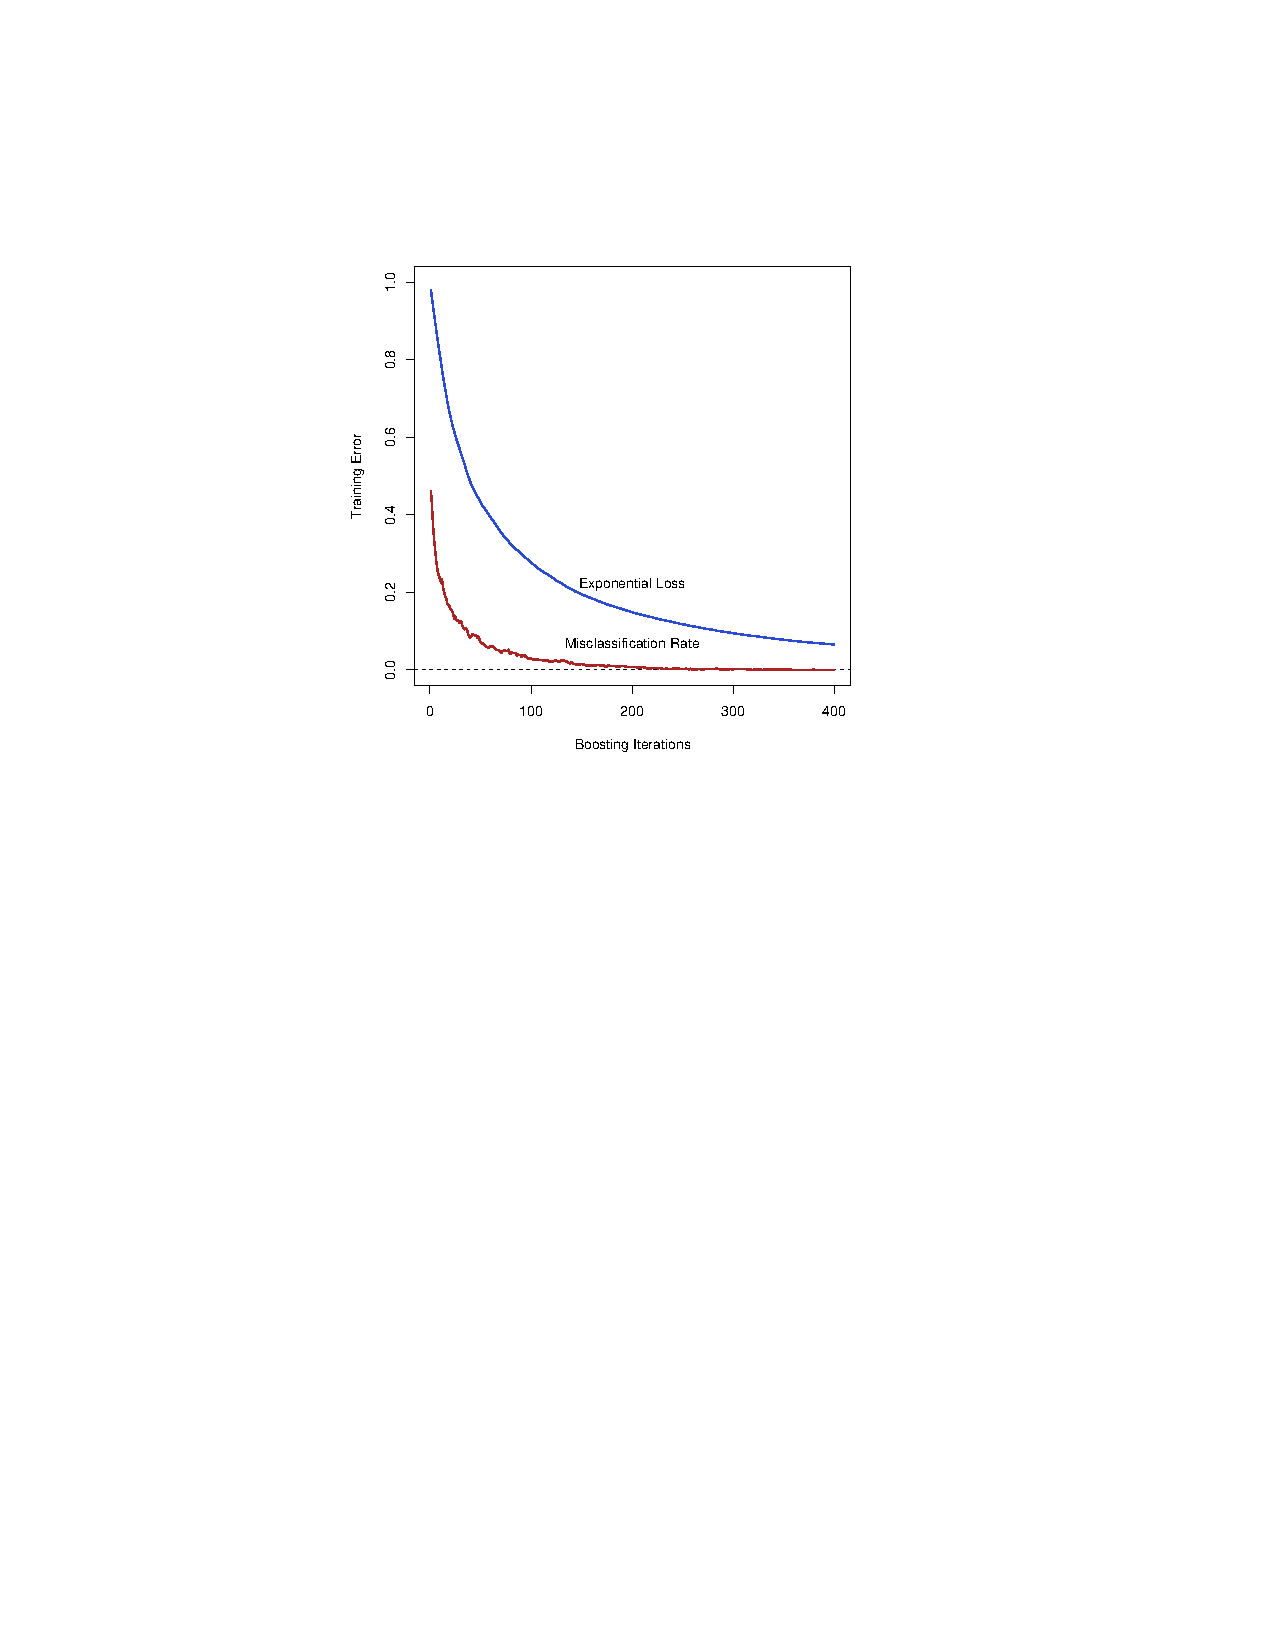
\includegraphics[width=0.6\textwidth]{figs/adaboost_expLoss}
	\\
	\cite{HastieEtAl2009}
\end{center}
\end{frame}

\begin{frame}[allowframebreaks]{AdaBoost}{Margins \& Overfitting}
\begin{itemize}[<+>]
	\item \alert{Margin} in boosting iteration $ k $ for example $ i $
	\begin{gather*}
		\gamma_{k, i} \triangleq y_i H_k\left(\mv x_i\right)
	\end{gather*}
	
	\item Assume zero training error: $ \gamma_{k, i} > 0 $, $ \forall i $
	
	\item Exponential loss $ E_k = \sum_{i=1}^N e^{-\gamma_{k, i}} $ can still be reduced!
	
	\item Loss reduces more sharply for examples with smaller $ \gamma_{k, i} $
	
	\only<.>{\centering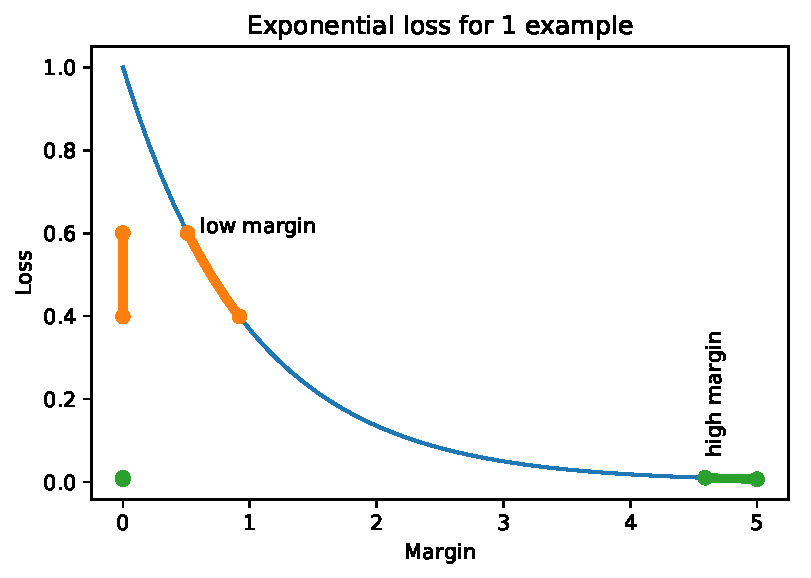
\includegraphics[width=0.5\textwidth]{figs/exp_loss}}
	
	\item AdaBoost tends to increase worst-case margin $ \min_i \gamma_{k, i} $
	
	\item<+-> How does AdaBoost avoid overfitting?
	\begin{itemize}[<.>]
		\item Stagewise addition of new learners makes learning slow
		\item Impact of change is localized as iterations procees
		\item Worst-case margin is pushed up (?)
	\end{itemize}
%	\item Typical weak learners:
%	\begin{itemize}[<.>]
%		\item decision stumps $ h(\mv x; j, s, \theta) = \sign\left( s (x_j - \theta) \right) $
%		\item perceptron $ h(\mv x; \mvs\uptheta, b) = \sign(\omega^\tp \mv x + b) $
%	\end{itemize}
\end{itemize}
\end{frame}

\begin{frame}{AdaBoost}{Why exponential loss?}
\begin{itemize}[<+>]
	\item Expected exponential loss is minimized for
	\begin{gather*}
		H^*(\mv x) = \argmin_{H(\mv x)} \E_{Y\cond \mv x} e^{-YH(\mv x)}
	\end{gather*}
	
	\item For binary classification with $ Y = \pm 1 $
	\begin{gather*}
		\E_{Y\cond \mv x} e^{-YH(\mv x)} = \Pr(Y=1\cond\mv x) e^{-H(\mv x)}
		+ \Pr(Y=-1\cond\mv x) e^{H(\mv x)}
	\end{gather*}
	
	\item Differentiating w.r.t\ $ H(\mv x) $ and setting to zero gives
	\begin{gather*}
		H^*(\mv x) = \frac{1}{2} \ln \frac{\Pr(Y=1\cond\mv x)}{\Pr(Y=-1\cond\mv x)}
	\end{gather*}
	
\end{itemize}
\end{frame}

\begin{frame}
\begin{itemize}[<+>]
	\item Now, assume $ Y\sim\BernDist(\phi(\mv x)) $ with 
	\begin{gather*}
		\phi(\mv x) = \frac{1}{1 + e^{-H(\mv x)}}
	\end{gather*}
	
	\item Negative log-likelihood loss is given by
	\begin{gather*}
		-l\left(H(\mv x)\right) = -\ln \left(1 + e^{-YH(\mv x)}\right)
	\end{gather*}
	
	\item Population minimizer is the same as for exponential loss
	\begin{gather*}
		\argmin_{H(\mv x)} \E_{Y\cond \mv x} e^{-YH(\mv x)}
		= \argmax_{H(\mv x)} \E_{Y\cond \mv x} l\left(H(\mv x)\right)
	\end{gather*}
	
	\item Equivalence does not hold for finite data sets!
\end{itemize}
\end{frame}

\begin{frame}
\centering
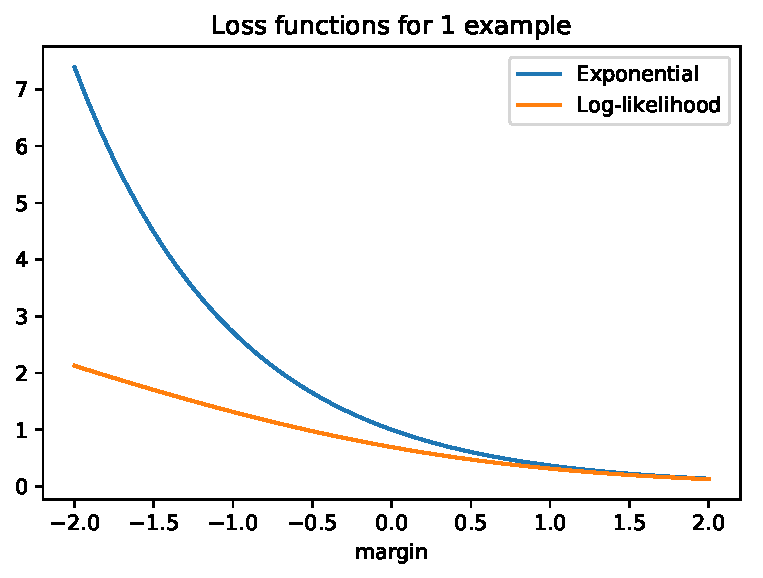
\includegraphics[width=0.7\textwidth]{figs/exp_ll_losses}
\begin{itemize}[<+>]
	\item Exponential loss puts more emphasis on misclassified examples
	\item Log-likelihood loss is more robust if
	\begin{itemize}[<.>]
		\item Bayes error rate is high
		\item there are mislabeled data
	\end{itemize}
\end{itemize}
\end{frame}



\section{Variants of AdaBoost}
\begin{frame}{Real AdaBoost \cite{FriedmanEtAl2000}}
\begin{itemize}[<+>]
	\item Initialization: $ \omega_1^{(1)} = \cdots = \omega_1^{(N)} = 1/N $
	\item<+-5> For $ k = 1, \ldots, K $ (until convergence)
	\begin{enumerate}[<+,6->]
		\item Fit classifier to target
		\begin{gather*}
			p_k(\mv x) = \hat P_\omega(Y=1\cond\mv x)
		\end{gather*}
%		\\
%		e.g.\ my maximizing
%		\begin{gather*}
%			\sum_{i=1}^N \omega_k^{(i)} \ln\left(
%				1 + e^{-y_i h_k(\mv x_i)}
%			\right)
%		\end{gather*}
		
		\item $ k $-th weak learner outputs
		\begin{gather*}
			h_k(\mv x) = \frac{1}{2} \ln\frac{p_k(\mv x)}{1-p_k(\mv x)}
		\end{gather*}
		
		\item Update and re-normalize the weights
		\begin{gather*}
			\omega_{k+1, i} \propto 
			\omega_{k, i} \exp\left[-y_i h_k(\mv x_i)\right],
			\qquad
			\sum\nolimits_{i=1}^N \omega_{k+1, i} = 1
		\end{gather*}
	\end{enumerate}
	\item Ensemble output is
	\begin{gather*}
		H_K(\mv x) = \sign\left( \sum\nolimits_{k=1}^K h_k(\mv x) \right)
	\end{gather*}
\end{itemize}
\end{frame}

\begin{frame}{LogitBoost \cite{FriedmanEtAl2000}}
\begin{itemize}[<+>]
	\item Additive logistic regression models.
	
	\item Newton optimization of the Bernoulli log-likelihood.

	\item Start with $ H(\mv x) = 0 $, $ \omega_{1:N} = 1/N $ and $ p(\mv x_i) = 1/2 $
	
	\item At iteration $ k $, compute the weights and ``working responses''
	\begin{align*}
		\omega_{i} = p(\mv x_i)\left(1 - p(\mv x_i)\right),
		\quad
		z_{i} = \min\left\{
			\frac{\indFun\{y_i=1\} - p(\mv x_i)}{\omega_{i}}, z_\text{max} 
		\right\}
	\end{align*}
	
	\item Find $ h_k(\mv x) $ via weighted least-squares
	\begin{gather*}
		h_k(\mv x) = \argmin_{h(\mv x)} \sum\nolimits_{i=1}^N 
			\omega_{i}\left[ z_i - h(\mv x_i) \right]^2
	\end{gather*}
	
	\item Update strong learner and probabilities
	\begin{gather*}
		H(\mv x) \leftarrow H(\mv x) + \frac{1}{2} h_k(\mv x), \quad
		p(\mv x) \leftarrow \frac{e^{H(\mv x)}}{e^{-H(\mv x)} + e^{H(\mv x)}}
	\end{gather*}
\end{itemize}
\end{frame}

\begin{frame}{Other AdaBoost modifications}
\begin{itemize}[<+>]
	\item Gentle AdaBoost \cite{FriedmanEtAl2000}
	\begin{itemize}[<.->]
		\item Real AdaBoost + Newton steps
		\item weighted least-squares regression instead of $ \Pr $ estimates
		\item more stable: no computation of log-ratios
	\end{itemize}

	\item LPBoost \cite{DemirizEtAl2002}
	\begin{itemize}[<.->]
		\item maximizes margin between classes
		\item learning is formulated as a linear programming problem
		\item totally corrective: weights of all past WLs are updated
	\end{itemize}

	\item Brown Boost \cite{Freund2001}
	\begin{itemize}[<.->]
		\item ``gives up'' on repeatedly misclassified examples
		\item robust to misslabeled datasets
	\end{itemize}

	\item Many many more \cite{FerrFigu2012}
\end{itemize}
\end{frame}



\section{Gradient Boosting}
\begin{frame}[allowframebreaks]{Gradient Boosting}{Toy example: sinusoidal regression}
	\centering
	\only<+>{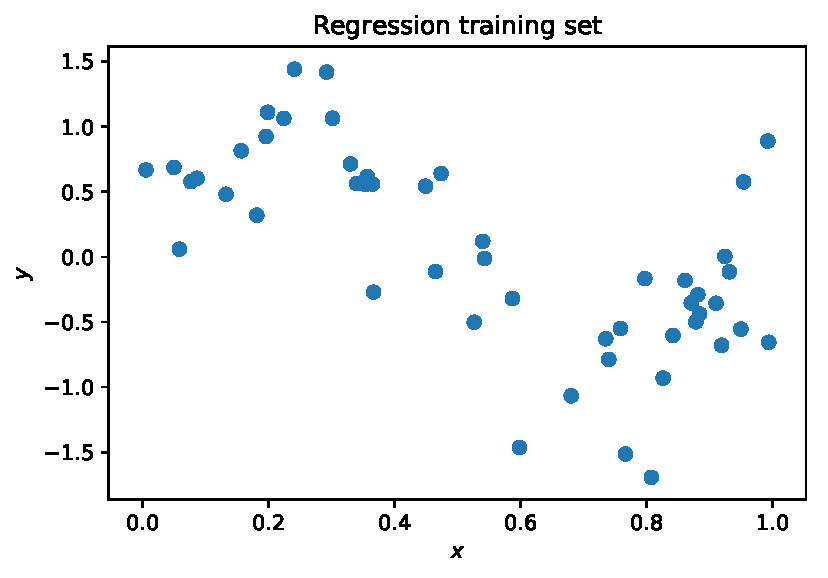
\includegraphics[width=0.9\textwidth]{figs/grad_boost_train_set}}
	\framebreak
	
	\only<+>{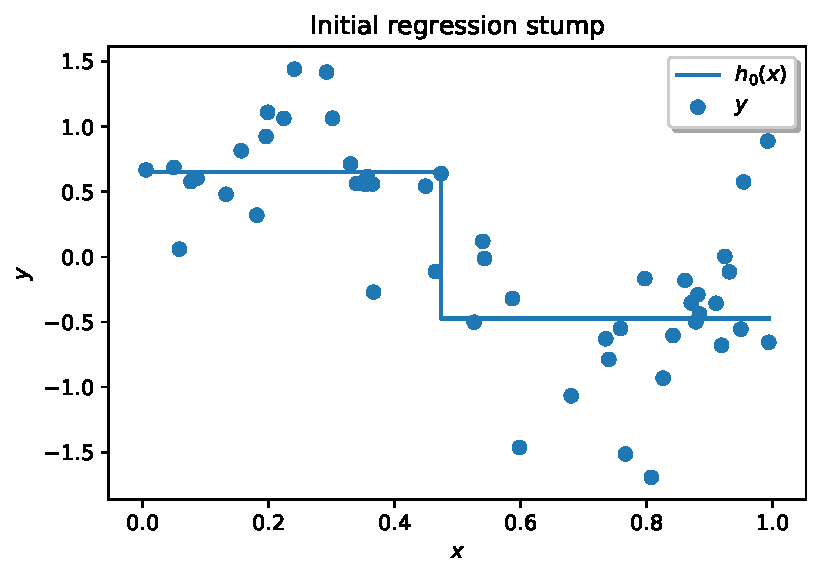
\includegraphics[width=0.9\textwidth]{figs/grad_boost_init}}
	\framebreak
	
	\only<+>{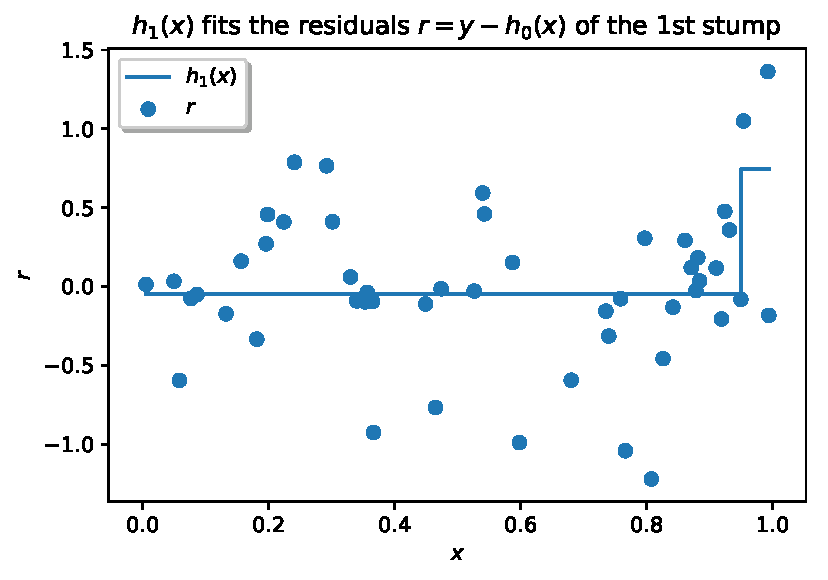
\includegraphics[width=0.9\textwidth]{figs/grad_boost_res}}
	\framebreak
	
	\only<+>{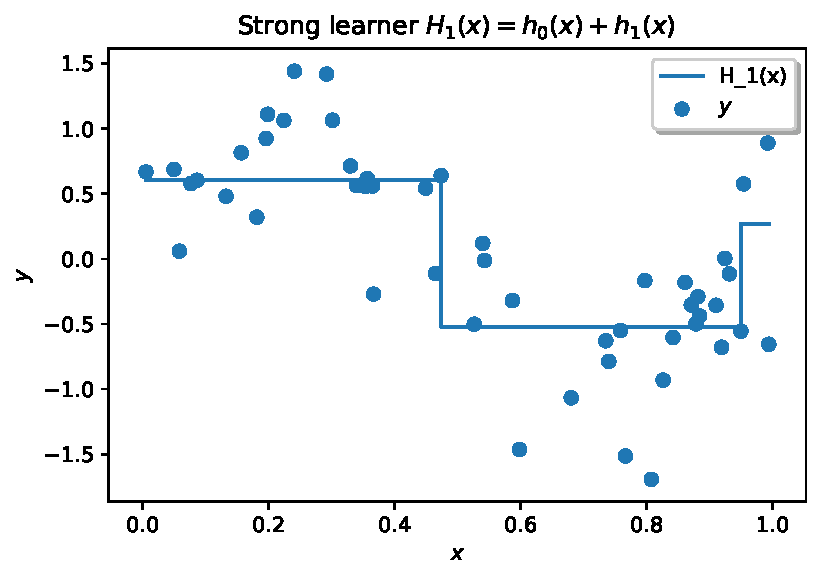
\includegraphics[width=0.9\textwidth]{figs/grad_boost_H1}}
	\framebreak
	
	\only<+>{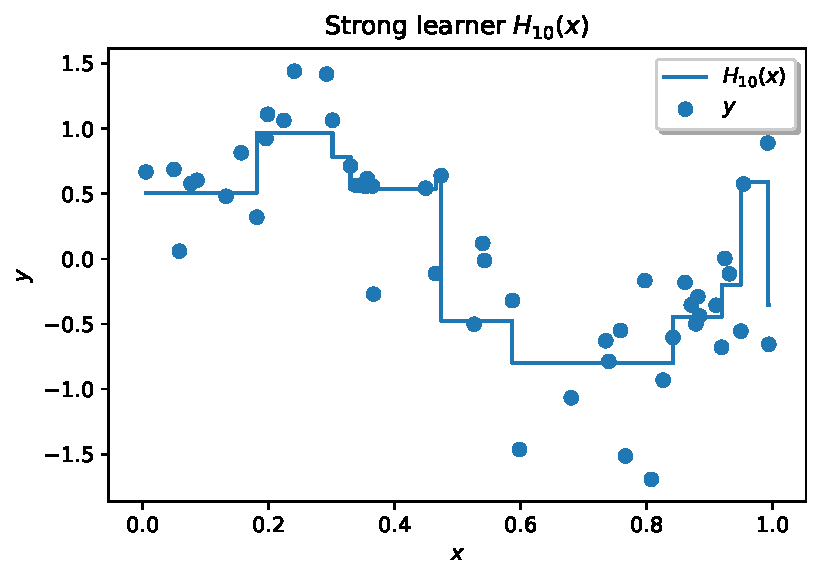
\includegraphics[width=0.9\textwidth]{figs/grad_boost_H10}}
\end{frame}

\begin{frame}{Why does residual fitting work?}
\begin{itemize}[<+>]
	\item Typical ML task: find $ H(\mv x) $ to minimize loss $ L(y, H(\mv x)) $.
	\item Generally unfeasible. Let's try a stagewise additive approach.
	\item Start with some simple $ H(\mv x) = h_0(\mv x) $ (e.g.\ regression stump).
	\item Add $ h_1(\mv x) $ to minimize resulting loss:
	\begin{gather*}
		h_1^*(\mv x) = \argmin_{h(\mv x)} L\left[
			y, H(\mv x) + h(\mv x)
		\right]
	\end{gather*}
	\item Gradient tells us where to go! Ideally,
	\begin{align*}
		g(\mv x) &\triangleq \left[
			\frac{\partial L(y, h)}{\partial h}
		\right]_{h = H(\mv x)}
		\\
		h_1(\mv x) &= - g(\mv x) 
		\tag{\text{optimal direction}}
		\\
		\alpha_1 &= \argmin_{\alpha} L\left[
			y, H(\mv x) + \alpha h_1(\mv x)
		\right]
		\tag{\text{optimal step size}}
	\end{align*}
\end{itemize}
\end{frame}

\begin{frame}
\begin{itemize}[<+>]
	\item But loss is evaluated on $ \{ y_i, \mv x_i \}_{i=1}^N $ and setting
	\begin{gather*}
		h_1(\mv x_i) = - g(\mv x_i)
		\quad
		\text{simultaneously for each $ i $}
	\end{gather*}
	is too hard (and would amount to overfitting, anyway)

	\item Approximate solution: try to fit the negative gradient
	\begin{gather*}
		\text{train $ h_1(\mv x) $ to minimize }
		\sum_{i=1}^{N} \left[
			-g(\mv x_i)	- h_1(\mv x_i)
		\right]^2
	\end{gather*}
	i.e.\ do a regression with negative gradient as target.
	
	\item For our sinusoidal regression toy example
	\begin{align*}
		L\left[
			y, H(\mv x)
		\right]
		&= \frac{1}{2} \left[
			y - H(\mv x)
		\right]^2
		\\
		-g(\mv x) &= y - H(\mv x)
	\end{align*}
	This is why residual fitting works!
\end{itemize}
\end{frame}

\begin{frame}{Typical loss functions}
\begin{itemize}[<+->]
	\item Huber loss is less sensitive to outliers
	\begin{gather*}
		L\left[ y, H(\mv x) \right] = \begin{cases}
			\left( y - H(\mv x) \right)^2/2, 
				& |y-H(\mv x)|\le \delta \\
			\delta\left( |y-H(\mv x)| - \delta \right)
		\end{cases}
	\end{gather*}
	\begin{center}
		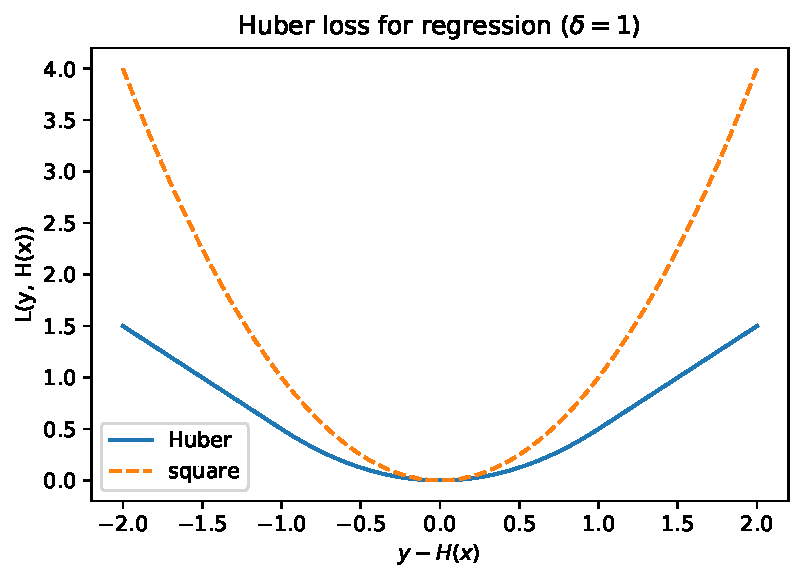
\includegraphics[width=0.5\textwidth]{figs/Huber_loss}
	\end{center}
	
	\item What about classification? Cross-entropy loss.
\end{itemize}
\end{frame}

\begin{frame}{Gradient tree boosting}
\begin{enumerate}
	\setcounter{enumi}{-1}
	\item<+> Start with $ H_0(\mv x) = \argmin_{\chi} \sum_{i=1}^{N} L(y_i, \chi) = \text{const.} $
	\item<+-6> For $ k = 1, \ldots, K $ (until convergence)
	\begin{enumerate}[<+, 7->][a)]
		\item Compute ``pseudo-residuals'' $ r_{k, i} = - g(\mv x_i) $
		\item Fit a regression tree on $ \{ \mv x_i, r_{k, i} \} $. This partitions input space into regions $ R_{k, 1} $, \ldots, $ R_{k, J_k} $
		\item Compute best output for each region
		\begin{gather*}
			\chi_{k, j} = \argmin_{\chi} \sum_{\mv x_i\in R_{k, j}}
				L\left[ y_i, H_{k-1}(\mv x_i) + \chi \right]
		\end{gather*}
		\item Update strong learner
		\begin{gather*}
			H_k(\mv x) = H_{k-1}(\mv x) 
			+ \sum_{j=1}^{J_k} \chi_{k, j} 
				\indFun\{ \mv x\in R_{k, j} \}
		\end{gather*}
	\end{enumerate}
	\item<+> Output $ H_K(\mv x) $ as final model.
\end{enumerate}
\end{frame}

\begin{frame}{Gradient tree boosting for classification}
\begin{itemize}
	\item Similar as for regression.
	
	\item $ M-1 $ trees for $ M $ classes, outputting $ f_{1:{M-1}}(\mv x) $
	\begin{align*}
		p_m(\mv x) &= \hat P(Y = m\cond \mv x) 
		\\
		&= \begin{cases}
			\dfrac{e^{f_m(\mv x)}}{1+\sum_{l=1}^{M-1} e^{f_l(\mv x)}},
				& m = 1, \ldots, M-1
			\\
			1 - \sum_{l=1}^{M-1} p_l(\mv x), & m = M
		\end{cases}
	\end{align*}
	
	\item Cross-entropy (deviance) loss
	\begin{align*}
		L(y, p(\mv x)) &= - \sum_{m=1}^{M} \indFun\{ y = m \} \ln p_m(\mv x)
		\\
		\frac{\partial L(y, p(\mv x))}{\partial p(\mv x)}
		&= \sum_{m=1}^{M} \indFun\{ y = m \} - p_m(\mv x)
	\end{align*}
\end{itemize}
\end{frame}

\begin{frame}{Gradient tree boosting hyper-parameters}
\begin{itemize}[<+>]
	\item Size of trees
	\begin{itemize}[<.->]
		\item controls amount of interactions between inputs
		%\item $ J = 2 $: decision stump---no interactions
		\item ``experience indicates $ 4 \le J \le 8 $'' \cite{HastieEtAl2009}
	\end{itemize}
	
	\item Number of iterations $ K $
	\begin{itemize}[<.->]
		\item large $ K $ leads to over-fitting
		\item chosen through early stopping
	\end{itemize}

	\item Shrinkage
	\begin{gather*}
		H_k(\mv x) = H_{k-1}(\mv x) 
		+ \alert{\nu} \sum\nolimits_{j=1}^{J} \chi_{k, j} \indFun\{ \mv x\in R_{k, j} \}
	\end{gather*}
	\begin{itemize}[<.->]
		\item smaller $ \nu $ = less overfitting, but requires larger $ K $
		\item set $ \nu < 0.1 $ and choose $ K $ via early stopping \cite{Friedman2001}
	\end{itemize}
	
	\item Subsampling (``stochastic gradient boosting'')
	\begin{itemize}[<.->]
		\item sample w/o replacement a fraction of $ \eta $ training examples
		\item grow $ k $-th tree using this sample
		\item poor performance without shrinkage
	\end{itemize}
\end{itemize}
\end{frame}

\begin{frame}{XGBoost}
	\begin{itemize}[<+>]
		\item Fast implementation of gradient boosted trees.
		
		\item Reduces search space of possible splits using the distribution of features across all examples in each leaf.
		
		\item Additional regularization---objective in iteration $ k $ is
		\begin{gather*}
			\underbrace{\sum_{i=1}^N L\left[
				y_i, H_{k-1}(\mv x_i) + h_k(\mv x_i)
			\right]}_\text{loss}
			+ \underbrace{\gamma T_k 
				+ \frac{\lambda}{2} \sum_{j=1}^{T_k} \omega_{k, j}^2
				+ \alpha \sum_{j=1}^{T_k} |\omega_{k, j}|}_\text{regularization}
		\end{gather*}
		\begin{tabular}{cl}
			$ T_k $ & number of leafs in $ k $-th tree \\
			$ \omega_{k, j} $ & output value (weight) in $ j $-th leaf
		\end{tabular}
	
		\item Uses 2nd order Taylor expansion of the objective
	
		\item Resources:
		\begin{itemize}[<.>]
			\item Tianqi Chens paper \cite{ChenGuestrin2016} and slides (\href{https://homes.cs.washington.edu/~tqchen/pdf/BoostedTree.pdf}{2014}, \href{https://speakerdeck.com/datasciencela/tianqi-chen-xgboost-overview-and-latest-news-la-meetup-talk}{2016})
			
			\item web \href{https://xgboost.ai/}{xgboost.ai}, github repo \href{https://github.com/dmlc/xgboost}{dmlc/xbgoost}
		\end{itemize}
	\end{itemize}
\end{frame}



\section{Concluding remarks}
\begin{frame}{Some success stories}
	\begin{itemize}[<+>]
	\item Fruend \& Schapire won the 2003 G\"{o}del Prize for AdaBoost.
		
	\item Viola-Jones object detection framework \cite{ViolaJones2001}
	\begin{itemize}[<.->]
		\item 1st framework with competitive detection rates in real-time
		\item AdaBoost with Haar features
	\end{itemize}

	\item Many more successful AdaBoost applications in \cite{FerrFigu2012}
	
	\item Yahoo \cite{CossockEtAl2008}, Yandex (\href{http://romip.ru/russir2009/slides/yandex/lecture.pdf}{slides}): gradient boosting for ranking
	
	\item XGBoost
	\begin{itemize}[<.->]
		\item Higgs Machine Learning Challenge \cite{ChenHe2015}
		
		\item ``Dominates structured or tabular datasets on classification and regression predictive modeling'' [\href{https://machinelearningmastery.com/gentle-introduction-xgboost-applied-machine-learning/}{machinelearningmastery.com}]
		
		\item \href{<https://github.com/dmlc/xgboost/tree/master/demo\#machine-learning-challenge-winning-solutions>}{List} of ML competition winning solutions
		
		\item Very popular on Kaggle
	\end{itemize}

	\end{itemize}
\end{frame}

\begin{frame}{Implementations}
	\begin{itemize}
		\item AdaBoost
		\begin{itemize}
			\item available in C++, Matlab, Python, R
			\item see \href{https://en.wikipedia.org/wiki/AdaBoost\#Implementations}{wikipedia entry}
		\end{itemize}
		
		\item Gradient Boosting
		\begin{itemize}
			\item Python/sklearn
			\item R (as Generalized Boosting Model)
		\end{itemize}
		
		\item XGBoost 
		\begin{itemize}
			\item Available for C++, Java, Python, R, Julia on Windows/Mac/Linux
			\item Support integration with scikit-learn
			\item Can be integrated into Spark, Hadoop, Flink
			\item see \href{https://en.wikipedia.org/wiki/Xgboost}{wikipedia entry} and \href{https://github.com/dmlc/xgboost}{github repo}
		\end{itemize}
	\end{itemize}
\end{frame}

\begin{frame}{Concluding remarks}
	\begin{itemize}[<+>]
		\item Pros of gradient boosted trees
		\begin{itemize}[<.->]
			\item naturally handles data of mixed types
			\item can handle missing values
			\item computationally scalable 
			\item able to deal with irrelevant inputs
			\item feature importance assessment
			\item interpretability
		\end{itemize}
	
		\item Cons w.r.t.\ deep nets
		\begin{itemize}[<.->]
			\item lower predictive power
			\item cannot extract features
		\end{itemize}
	\end{itemize}

	\uncover<+>{\begin{quote}
		When in doubt, use xgboost
		[\href{http://blog.kaggle.com/2015/08/26/avito-winners-interview-1st-place-owen-zhang/}{Kaggle winner}]
	\end{quote}}
\end{frame}

\begin{frame}[allowframebreaks]{References}
	\bibliographystyle{alpha}
	%\bibliographystyle{apalike}
	%\bibliographystyle{plain}
	\bibliography{references}
\end{frame}

\end{document}